\documentclass{beamer}
\usepackage{lmodern}
\usepackage[frenchb]{babel}
\usepackage[T1]{fontenc}
\usepackage[utf8]{inputenc}
\usepackage{graphicx}
\usepackage{bm}
\usepackage{amsmath}

\addtobeamertemplate{navigation symbols}{}{%
\usebeamerfont{footline}%
\usebeamercolor[fg]{footline}%
\hspace{1em}%
\insertframenumber/\inserttotalframenumber
}


\usetheme{Warsaw}

\title{A Necessary and Sufficient Condition for
Consensus Over Random Networks}
\author{Jeremy Krebs - Guillaume Soulié}
\institute{Université Paris Saclay}
\date{\today}

\begin{document}

\begin{frame}
\titlepage
\end{frame}


\section{Introduction}
\begin{frame}
	\textbf{Le problème du consensus :}

	"Le consensus demande à ce qu'un certain nombre de processus s'accordent sur une valeur unique."
	\begin{center}
		\only<2>{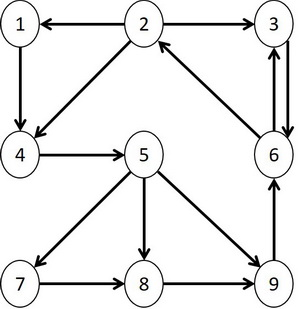
\includegraphics[width=3cm]{media/conv}}
		\only<3>{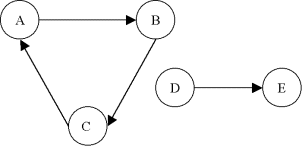
\includegraphics[width=5cm]{media/non_conv}}
	\end{center}
\end{frame}


\begin{frame}
	\tableofcontents
\end{frame}

\subsection{Etat de l'art}
\begin{frame}
		Le problème de consensus suscite beaucoup d'intérêt:
		 \begin{itemize}
		 	\item Coordination d'agents autonomes
		 	\pause
		 	\item Calculs de moyennes d'un groupe de capteurs
		 	\pause
		 	\item Problèmes de rendez-vous
		 \end{itemize}
		 
		 \pause
		 
		 Cependant ces problèmes considéraient un système déterministe.
\end{frame}		

\begin{frame}
	\begin{itemize}
		\item Temps discret: $t_0, t_1, ...$
		\item Systèmes stochastiques
	\end{itemize}
	
	\pause
	
	Problème de la forme:
	$ x_{k+1} = W_k . x_k $
	
	$W_k$ peut être vu comme la matrice de poids d'arêtes d'un graphe aléatoire.
\end{frame}

\begin{frame}
	Il y a déjà eu plusieurs résultats sur le sujet:
	\begin{itemize}
		\item $x(k)$ converge presque sûrement si les arêtes de $G(W_k)$ sont choisies de manière indépendante et avec la même probabilité,
		\pause
		\item La convergence en probabilité a été prouvée dans le cas d'un modèle avec des arêtes orientées et non-nécessairement indépendantes, avec une hypothèse un peu forte sur les matrices.
	\end{itemize}
\end{frame}

\subsection{Objectif}

\begin{frame}
	\textbf{Objectif}:
	\begin{itemize}
		\item Trouver une condition nécessaire et suffisante pour un consensus presque sûr
		\item S'intéresser à la valeur de convergence du consensus
	\end{itemize}
\end{frame}
		
\section{Préambule mathémathique}
\subsection{Définitions}
\begin{frame}
	$ x(k) = W_k(\omega)x(k-1)$ où $W_k$ est une matrice de poids.
	
	\begin{itemize}
		\item Les $W_k$ sont des matrices stochastiques indépendantes et identiquement distribuées (i.i.d.),
		\item $j$ a accès à $i$ si $(i,j)$ est une arête,
		\item $i$ et $j$ communiquent si $(i,j)$ et $(j,i)$ sont des arêtes,
		\item La relation de communication est une relation d'équivalence qui permet de regrouper les arêtes par classes d'équivalence.
	\end{itemize}
\end{frame}

\begin{frame}
	\textbf{Consensus en probabilité:}
	
	$\forall\ \epsilon > 0\ \forall\ i,j = 1,..,n\ P(|x_i(k) - x_j(k)| > \epsilon) \rightarrow 0$
	
	lorsque $k \rightarrow 0$
	
	\bigbreak
	
	\pause
	
	
	\textbf{Consensus presque sûr (plus forte):}
	
	$\forall\ i,j = 1,..,n\ |x_i(k) - x_j(k)|\rightarrow 0$ presque sûrement.
\end{frame}

\subsection{Ergodicité}
\begin{frame}
	$x_k = W_k ... W_1\ x_0$
	
	\bigbreak
	
	Intérêt d'étudier le produit infini de matrices $W_i$ et son ergodicité.
	
	\bigbreak
		
	Notons $U^{(k, p)} = W_{p+k}...W_{p+1}$ le produit à gauche des matrices de la séquence.
\end{frame}

\begin{frame}
	\textbf{Définition - Ergodicité faible:}
	
	La séquence infinie $W_1, W_2, ...$ est faiblement ergodique si et seulement si
	
	$ \forall\ i, j, s = 1,..,n\ $ et $\forall\ p > 0\ (U_{i,s}^{k,p} - U_{j,s}^{k,p}) \rightarrow 0$ quand $k \rightarrow \infty$
	
	\bigbreak

	\pause
	
	\textbf{Définition - Ergodicité forte:}
	
	La séquence infinie $W_1, W_2, ...$ est faiblement ergodique si et seulement si
	
	$ \forall\ i, s = 1,..,n\ U_{i,s}^{k,p} \rightarrow d_s^p$ quand $k \rightarrow \infty$
	
	où $d_s^p$ est une constante ne dépendant pas de $i$
	\\ backend
	\vspace{1cm}
	\pause
	Dans le contexte qui nous intéresse, on peut montrer (en utilisant les suites de Cauchy) 
	que les notions d'ergodicité faible et fortes sont équivalentes.
	
\end{frame}


\begin{frame}
	\textbf{Ergodicité - consensus}

	\begin{center}		
		$ x(k) = W_k \cdot x(k-1)$
	\end{center}

	\begin{equation}
		\nonumber
		\begin{pmatrix}
			x^k_0\\
			x^k_1\\
			...\\
			x^k_n
		\end{pmatrix}
		=
		\begin{pmatrix}
			w^k_{00} & ... & w^k_{0n}\\
			w^k_{10} & ... & w^k_{1n}\\
			... &  & ... \\
			w^k_{n0} & ... & w^k_{nn}
		\end{pmatrix}
		\cdot
		\begin{pmatrix}
			x^{k-1}_0\\
			x^{k-1}_1\\
			...\\
			x^{k-1}_n
		\end{pmatrix}
	\end{equation}
\end{frame}

\begin{frame}
	\textbf{Coefficient de d'ergodicité}
		Une fonction $\tau(.)$ définie sur l'ensemble des matrices stochastiques de taille $n \times n$ est un coefficient d'ergodicité si $0 \leq \tau(.) \leq 1$.
		\bigbreak
		\pause
		Un coefficient d'ergodicité est dît propre si:
		\begin{center}
			$\tau(W) = 0 \iff W = $ \textbf{1}$d^T$
		\end{center}
		\pause
		Example de coefficient d'ergodicité.
\end{frame}

\begin{frame}
	\textbf{Lien ergodicité faible - coefficient d'ergodicité}
	L'ergodicité faible est équivalente à:
	\begin{equation}
		\nonumber
		\lim_{k \to \inf} \tau(U^{(k, p)}) = 0 \quad \forall p \in \mathbb{N} 
	\end{equation}
\end{frame}


\begin{frame}
	\textbf{Théorème 1:}
		L'ergodicité faible du produit à gauche des matrices stochastiques est équivalente à son ergodicité forte.
	\bigbreak
	
	\pause

	\textbf{Théorème 2:}
		Si $\tau(.)$ est un coefficient d'ergodicité propre et que pour les $\forall m \geq 1$ matrices stochastiques $W_k,\ k=1,..,m$ on a $\tau(W_m .. W_2W_1) \leq \prod_{k=1}^m\tau(W_k)$,
		
	\pause	
	\bigbreak		
		
		Alors la séquence $W_k$ est faiblement ergodique si et seulement si il existe une séquence d'entiers croissants $k_r, k=1,2,..$ telle que :

			\bigbreak
			
			$\sum_{k=1}^{\infty}(1 - \tau(W_{k_{r+1}}..W_{k_r + 1}) = \infty$

\end{frame}

\section{Résultats}

\subsection{Condition nécéssaire et suffisante}


\begin{frame}
	\textbf{Lemme 1}
	
	L'ergodicité faible de $W_1, W_2, ... $ est un événement trivial.
	\bigbreak
	\pause
	La démonstration repose sur la loi du zéro un de Kolmorov.
	
	\pause
	\textbf{Théorème 3}
	\begin{center}
		$\{W_k\}_{k=0}^{\inf} = W_1, W_2, ...$ i.i.d. matrices stochastiques, 
		avec des coefficients diagonaux positifs.
		\pause
		Il y a équivalence entre:
		\begin{itemize}
			\item $\{W_k\}_{k=0}^{\inf}$ est faiblement ergodique.
			\pause
			\item Le système $x(k) = (\mathbb{E}W_k)x(k-1)$ atteint un consensus.
			\item $| \lambda_2(\mathbb{E}W_k)| < 1$
		\end{itemize}
	\end{center}
	\pause
	\bigbreak
	Sa démonstration peut être faite au choix:
	\begin{itemize}
		\item En utilisant des résultats généraux de la théorie ergodique des chaines de Markov.
		\item En utilisant le théorème 2.
	\end{itemize}
\end{frame}
\begin{frame}
	\textbf{Lemme 2} - (D'après [19])
	\begin{itemize}
		\item $\alpha_1, ..., \alpha_s$: classes de communication associées à $W$.
		\item $\alpha_r[W]$ est la sous matricede $W$ associée à $\alpha_r$
		\item alors $\alpha_r$ est initial $\iff$ $spectre(\alpha_r[W]) = \{1\}$.
	\end{itemize}
\end{frame}
\begin{frame}
	\textbf{Corrollaire 4 - (Résultat principal de l'article)}
	\begin{center}
		consensus presque surement atteint
		$\iff$
		$|\lambda_{2}(\mathbb{E}W_k)| < 1$
	\end{center}
	\pause
	\bigbreak
	=> vient généraliser certain papiers.
\end{frame}

	\subsection{Valeur du consensus}
\begin{frame}
	\textbf{Valeur du consensus}

	On a vu $| \lambda_2(\mathbb{E}W_k)| < 1$ implique $x \to c\textbf{1}$

	($c$ dépend de $x(0)$ et des matrices $W_k$.)

	\bigbreak
	\pause
	\textbf{Théorème 5}

	For $y \in \mathbb{R}$, posons $S(y) = \{W \in S_n | y^TW = y^T\}$

	si $| \lambda_2(\mathbb{E}W_k)| < 1$ et $\mu (S_n - s(y)) = 0$, alors

	\begin{center}
		$\lim_{k \to \inf}x(k) = (y^Tx(0))\textbf{1}$ \quad a.s.		
	\end{center}
	\pause
	Les matrices $W_k$ partagent le même vecteur propre de gauche
	(associé à la valeur propre 1).
\end{frame}


\section*{Conclusion}
\begin{frame}
	Ce que le papier apporte :
	\begin{itemize}
		\item Le problème du consensus peut être réduit à un problème de faible ergodicité.
		\pause
		\item Il est caractérisé par la valeur de la deuxième valeur propre de $\mathbb{E}W_k$.
		\pause
		\item Sous certaines conditions des $W_k$, on peut déterminer de manière certaines la valeur de consensus.
	\end{itemize}
	\pause
	Pour aller plus loin :
	\begin{itemize}
		\item Quelles sont les performances d'un tel consensus ?
		\pause
		\item Quelles réactions face aux perturbations ? (ajout d'un 'bruit de communication' stochastique, ...)
		\pause
		\item Que se passe-t-il si la topologie du graphe varie au cours du temps ?
	\end{itemize}
\end{frame}

\begin{frame}
	\begin{center}
		\LARGE Questions ?
	\end{center}
\end{frame}

\end{document}
